\section{Model and Assimilation}

\subsection{1D-ERSEM model}

We use a 1D coupled ERSEM model. The physical forcing comes from a 3D
circulation simulation of the Red Sea [Yao 2014]. The ecological models are
initialized with the results of the 3D Red Sea ecology simulation
[Triantfyllou2013].

\begin{quotation} The 1D regional ecological models used for this thesis have
been configured and are operational. Three models will be used: for the
northern, central and southern Red Sea. The extreme south of the Red Sea is not
modeled, as its dynamics is poorly understand and we miss in situ data.  The
ecology is modeled with ERSEM, and the hydrodynamics is modeled with the
MITgcm.

The results of the MITgcm are those from \citet{Yao2014, Yao2014b}, in which a
simulation of the Red Sea and part of the Gulf of Aden circulation was run over
50 years. The NCEP data were used for atmospheric forcing, and the ocean ECCO
data for the open boundary conditions in the Gulf of Aden. The output of the 50
years run are used for the temperature and vertical circulation at the modeled
points.

ERSEM simulates the complete water column with the pelagic and benthic
ecosystems, as well a their coupling. The equations model the flow of carbon,
nitrogen, phosphorus and silicon in the ecosystem. Living organisms are modeled
in terms of population processes (growth and mortality) and physiological
processes (ingestion, respiration, excretion, and egestion). The biota is
divided into functional groups according to their trophic levels: producers
(phytoplankton), consumers (zooplankton) and decomposers (bacteria), and
further subdivided according to their sizes \citep{Baretta1995}.

The ecological models are initialized with the results of a 3D ecological
simulation of the Red Sea \citep{Triantafyllou2014}. The nutrient
concentrations are initialized using values from the World Ocean Atlas 2005
(WOA 2005).  \end{quotation}

\subsection{Data Assimilation}

To improve the results of the simulation we use the hybrid-SEIK assimilation
scheme, detailed in this subsection.

\begin{quotation} The assimilation scheme for the ecological models has been
implemented and is operational. The chosen scheme is the hybrid-SEIK, described
in \citet{Hamill2000}. It can be seen as a variant of the 3DVAR variational
assimilation scheme. 3DVAR assumes that the error forecast covariance is fixed
in time. In the case of the hybrid, the covariance is a linear combination of
the 3DVAR covariance and the time-evolving SEIK covariance matrix. Figure
\ref{assim} shows the assimilation scheme improves the fit of the model to the
chlorophyll data.

The problem of optimal filtering can be solved exactly by the Kalman Filter for
linear systems. For nonlinear models, one can use the Extended Kalman (EK)
filter, in which the model is linearized by computing the error covariance
function.  However, when the state is large, as is often the case for
oceanographic applications, the EK is intractable. In that case, SEEK can be
used, where the error covariance function is projected into a smaller subspace.
This subspace evolves to ensure that most of the error is represented and
filtered out. SEIK can be viewed as an ensemble variant of the SEEK, where the
error covariance function is represented exactly by an ensemble of states. This
avoids the computation of model gradients, and allows the assimilation scheme
to perform better when this model is strongly non-linear. SEIK has been shown
to be efficient for large-scale 3D ecosystem simulations
\citep{Triantafyllou2003}.

%\begin{figure} \centering 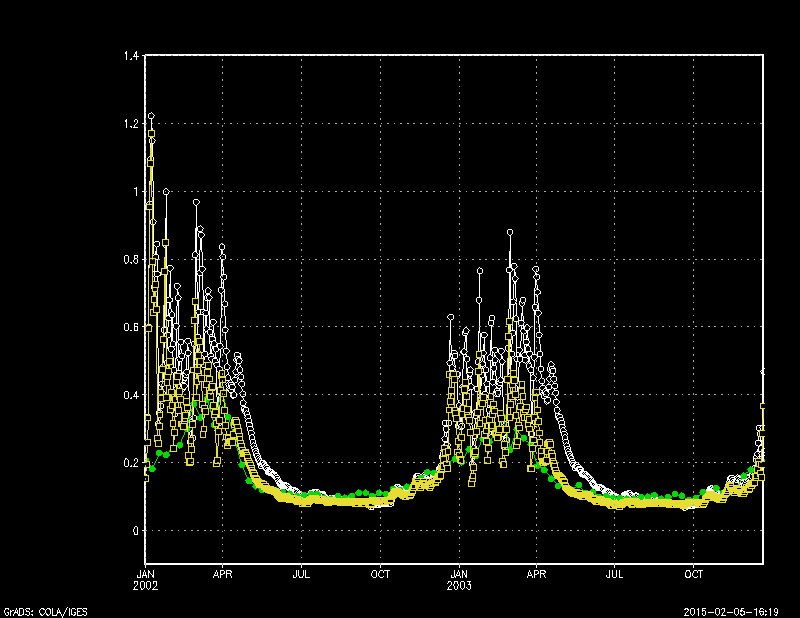
\includegraphics[scale=.45]{figures/chl_factor.png}
%\caption{Surface chlorophyll in the northern Red Sea from CCI data (green),
%from a free run of the 1D ecological model (white), with data assimilation
%(yellow)} \label{assim} \end{figure}

The Expectation-Maximization scheme to estimate the filter parameters has also
been derived. It is similar to that proposed by \citet{Tandeo2014}, except that
the model is non linear. The scheme will be used to improve the estimates of
the observation and model covariance errors.  \end{quotation}

